

Agora, além do vetor com as intensidades de vermelho, verde e azul, adicionamos também a coordenada x e y de cada pixel, com um certo peso w.

\begin{lstlisting}[language=Python]
def function_4(img, parameter, weight):
    tmp = img.copy()
    tmp = np.dstack((img, np.zeros((img.shape[0], img.shape[1]))))
    tmp = np.dstack((tmp, np.zeros((img.shape[0], img.shape[1]))))
    for i in range(tmp.shape[0]):
        for j in range(tmp.shape[1]):
            tmp[i, j, 3] = weight * i  # Coordenada x
            tmp[i, j, 4] = weight * j  # Coordenada y
    temp = np.reshape(tmp, (img.shape[0] * img.shape[1], 5))
    model = KMeans(n_clusters=parameter, random_state=0, n_init="auto").fit(temp)
    output = model.cluster_centers_[model.labels_]
    output = np.reshape(output, (img.shape[0], img.shape[1], 5))
    return output[:, :, :3]

# Teste com diferentes pesos
weights = [0, 0.001, 0.005, 0.0075, 0.01, 0.02, 0.05, 0.1, 1]
\end{lstlisting}

\begin{figure}[H]
    \centering
    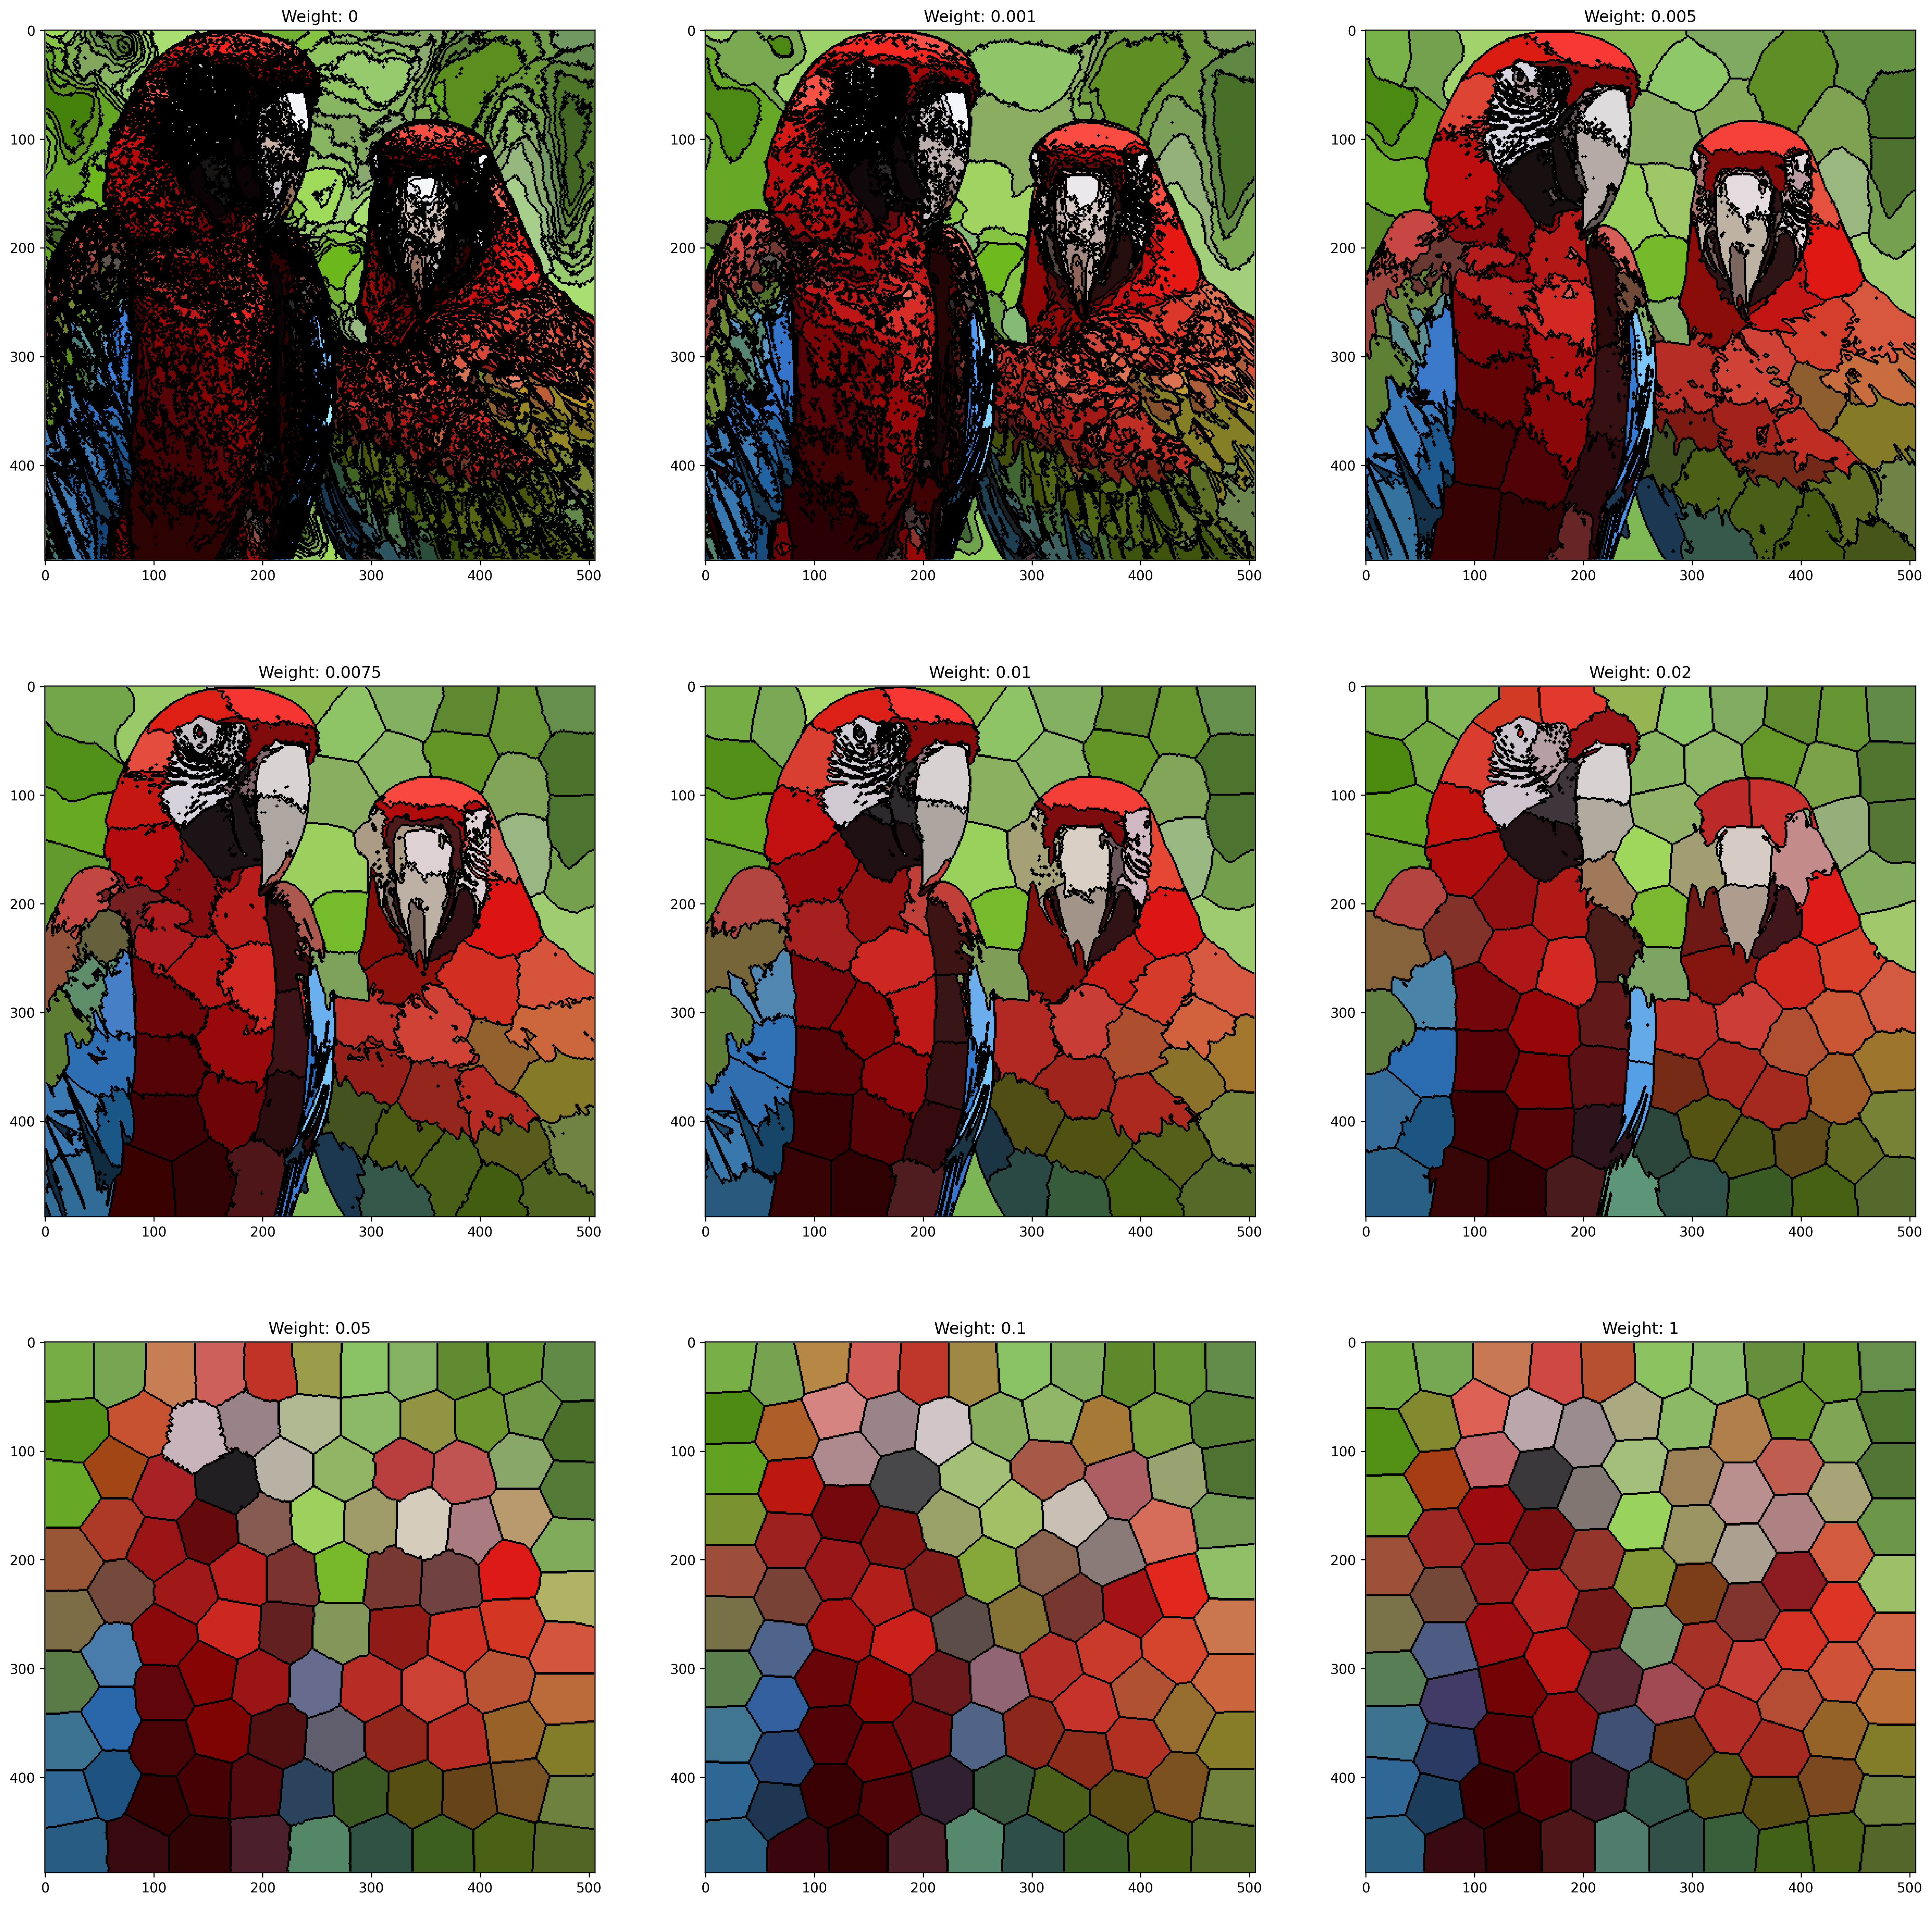
\includegraphics[width=0.9\textwidth]{../figures/5/weight_effects.png}
    \caption{Efeito do peso w na clusterização com coordenadas espaciais}
    \label{fig:weight_effects}
\end{figure}


A inclusão das coordenadas x e y adicionam informação espacial para o algoritmo de clusterização. Assim, além da similaridade das cores, ele também considerará
a proximidade entre os pixels. Os valores de w definem o quão sensível será o algoritmo à distância, de modo que valores pequenos de w fazem com que o método priorize
mais as cores, enquanto valores maiores dão enfoque na posição.

As figuras resultantes indicam exatamente isto. Para w = 0, temos o algoritmo original, apenas com cores, e para w maiores que 0.05, as cores praticamente não
importam, pois seus valores têm magnitude menor que a da posição de cada pixel. Nesta configuração, o contorno dos clusters é regular já que a fronteira entre os
grupos são basicamente os pontos equidistantes a dois ou, no caso das arestas entre três hexágonos, três centróides. Além disso, os centroides tendem a se organizar
em um formato regular, já que esta configuração seria mais adequada para aumentar a pureza entre os clusters.
